\chapter{The UAV control problem}\label{ch:UAVControlProblem}
\noindent This chapter specifies optimal control architecture for UAV and defines assumptions.
\section{The control problem}
\noindent \textit{Obstacle avoidance} in terms of control is complex optimisation problem with dynamic constraints. Movement constraints are mainly given by static uncharted obstacles and non-cooperative intruders. This work focus on uncharted obstacles. Non-cooperative intruders are omitted in this work. Usually multiple layer control concept is used. Control concept used for this work is in fig. \ref{fig:controlConceptIntro}.
\begin{figure}[H]
    \centering
    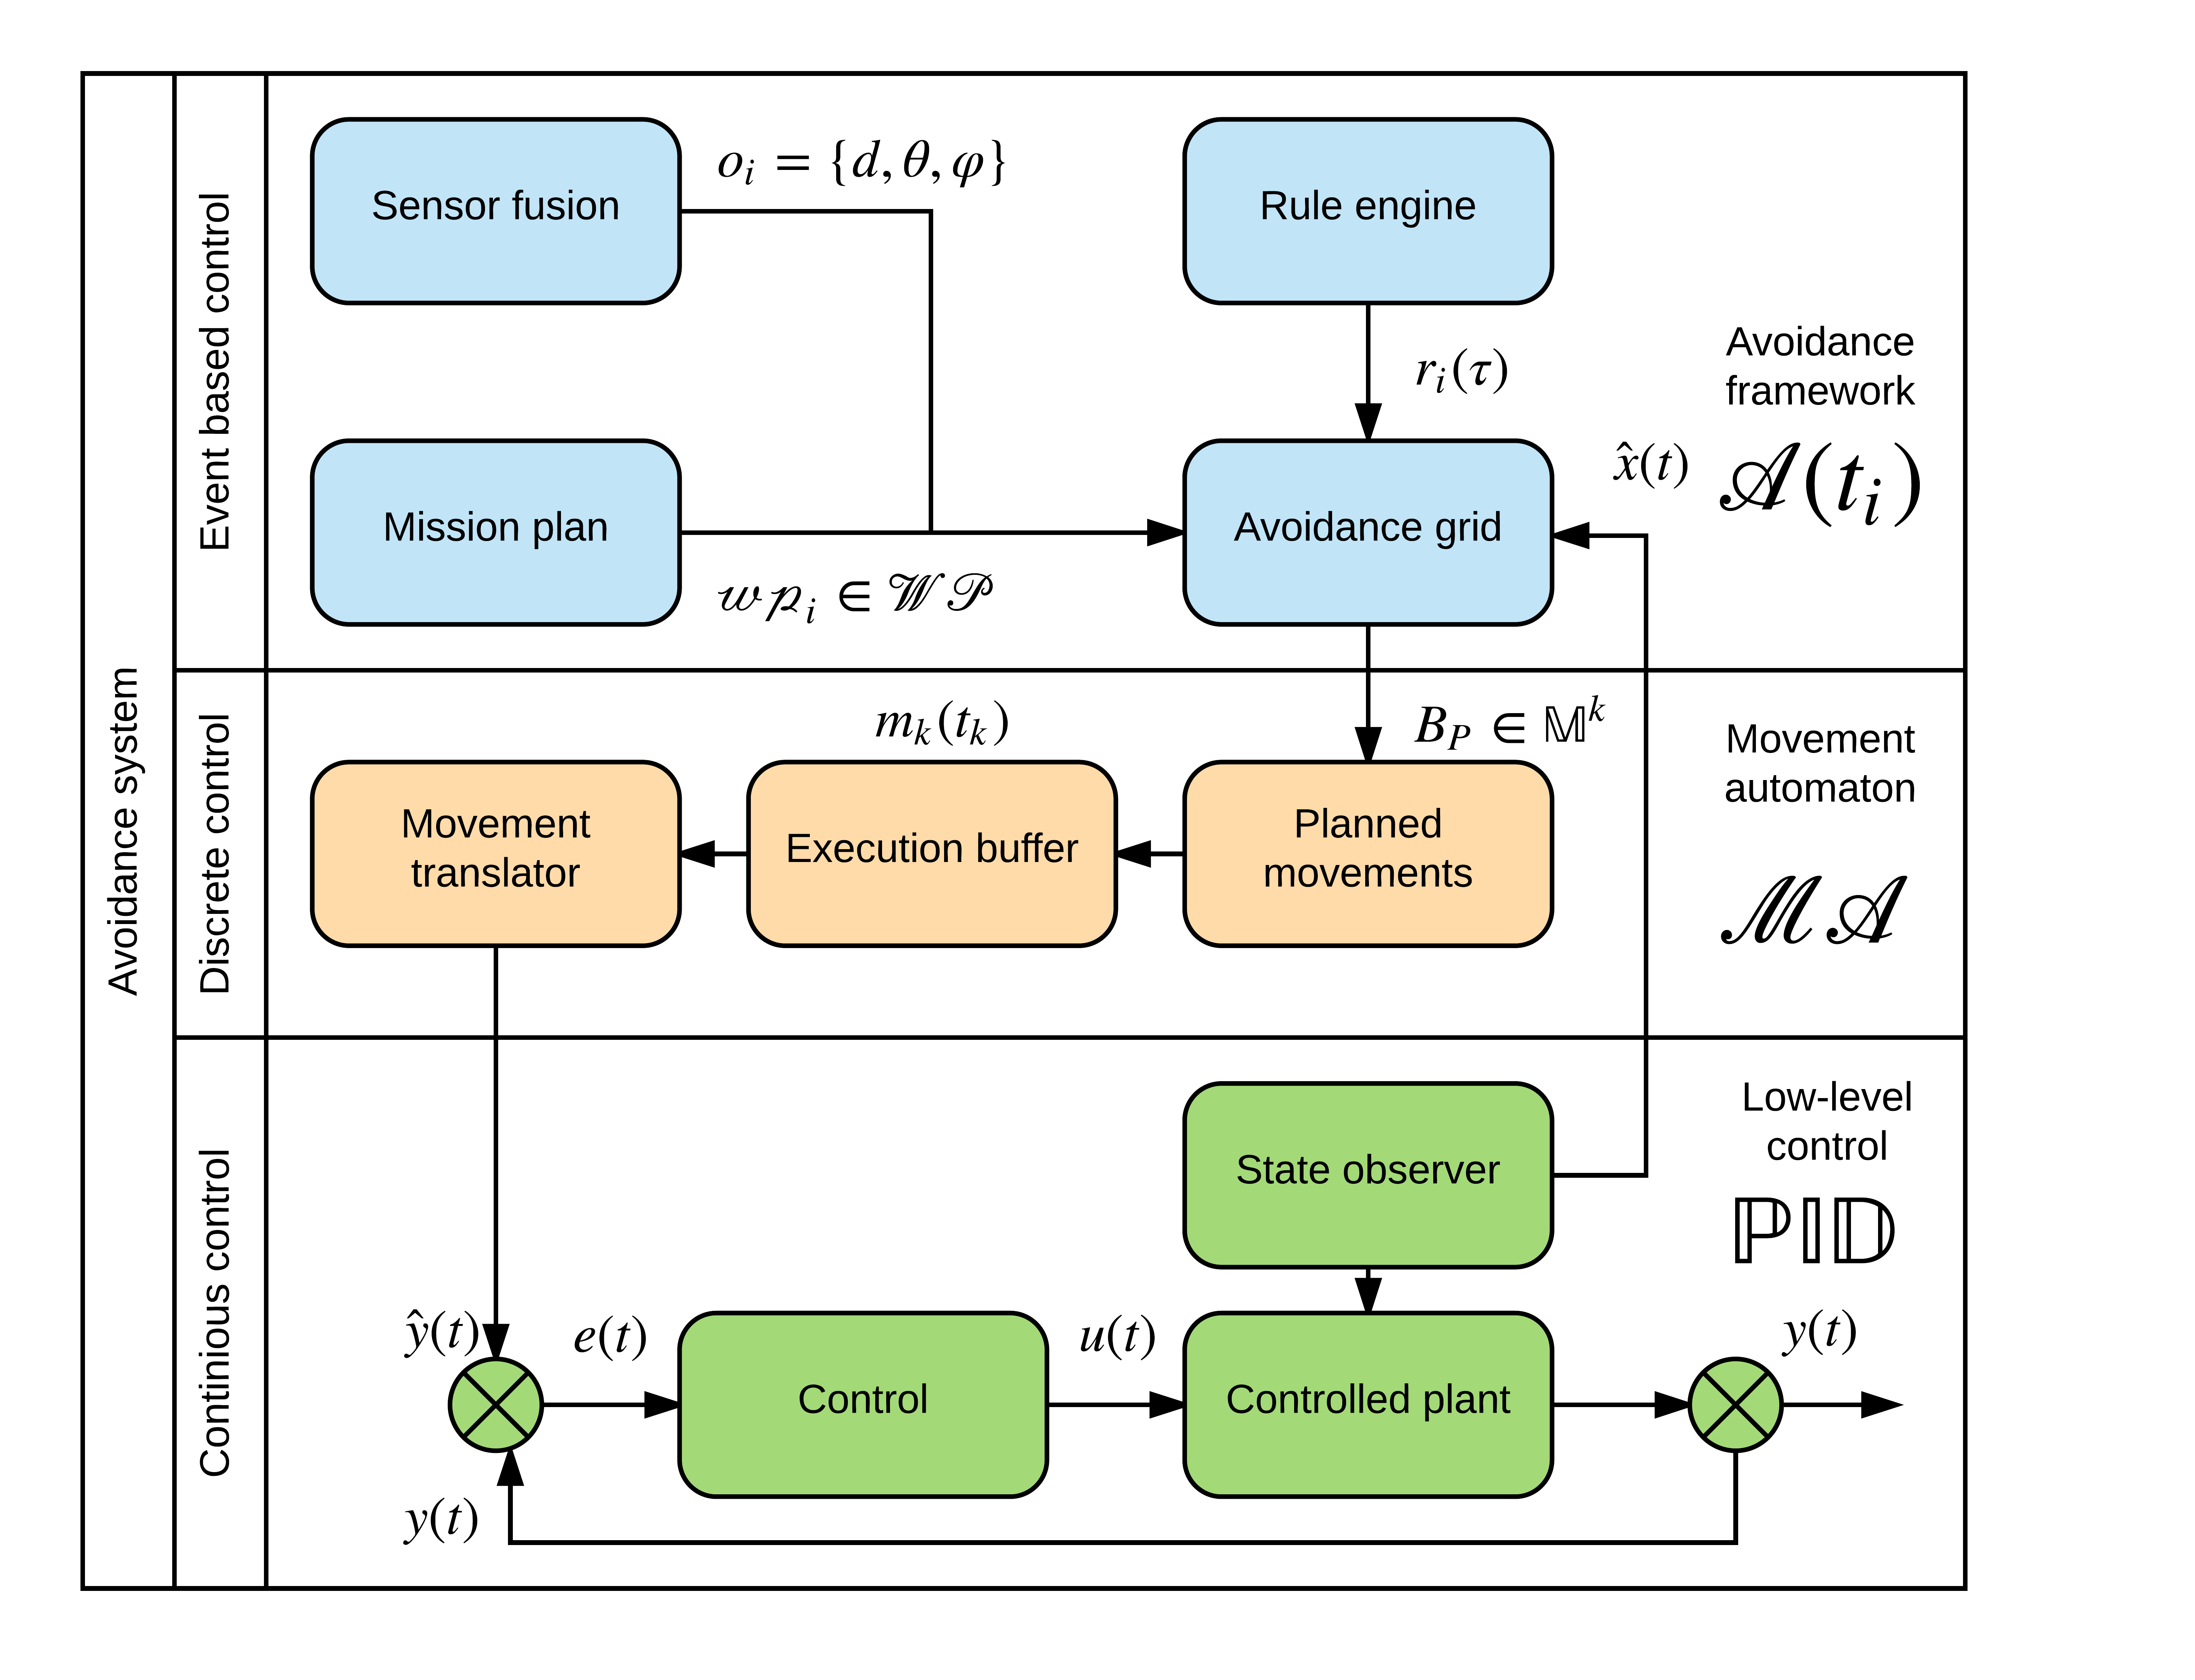
\includegraphics[width=.95\linewidth]{\FIGDIR/72_Control_Concept.png}
    \caption{Decision frame $\mathscr{D}(0)$.}
    \label{fig:controlConceptIntro}
\end{figure}

\noindent \textit{Event based control} module is responsible for high level decisions and mission execution. This module generates high level input commands which are optimal to given criterion. \textit{Event based control} consist from following artifacts:
\begin{enumerate}
    \item \textit{Sensor fusion} - fuses data from sensor system with observed system state $\hat{x}$, outputs detected obstacles $o_i\in\mathscr{O}$.
    \item \textit{Mission plan} - contains mission plan $\mathscr{WP}$, determines navigation goal waypoint $\mathscr{WP}_g$.
    \item \textit{Rule engine} - determines additional constraints for avoidance grid $\mathscr{A}(t_i)$, determines escape goal in avoidance grid $c_{i,j,k}$.
    \item \textit{Avoidance grid} - responsible for optimal path planning in partially known space, consumes observed system state $\hat{x}(t)$, rule engine decisions $r_i(\tau)$, obstacle set $o_i\in\mathscr{O}$ and goal waypoint $\mathscr{WP}_i$, produces avoidance command chain $B_p \in \mathbb{M}^k$.
\end{enumerate}

\noindent \textit{Discrete control} module is responsible for processing high level movement command chain $B_p \in \mathbb{M}^k$. It is implemented as special type of open hybrid automaton, movement automaton $\mathscr{MA}$. Movement automaton $\mathscr{MA}$ have following notable artifacts:
\begin{enumerate}
    \item \textit{Planned movements} - buffers planned movements from avoidance grid $B_P\in\mathbb{M}^k$, planed movements buffer can be extended by additional movements (normal situation) or filled with new movement chain(flush) in case of trajectory correction or avoidance. Planned movement is similar to FIFO stack.
    \item \textit{Execution buffer} - executes first command from \textit{planned movements}, based on previous movement $m_{k-1}(t_{(k-1)})$ and actual command $m_k(t_k)$ chain of movement primitives $\{p_1, \dots p_l\}$ is created. Chain of movement primitives $\{p_1, \dots p_l\}$ is forwarded to movement translator.
    \item \textit{Movement translator} - translates chain of movement primitives or other movement representation to:
    \begin{enumerate}[a.]
        \item \textit{Desired input signal $\hat{u}(t),t\in<t_{(k-1)},t_k)$,} - in case of \textit{open loop control}, in this case desired control signal is feed directly to \textit{controlled plant}.
        \item \textit{Desired output signal $\hat{y}(t),t\in<t_{(k-1)},t_k)$} - in case of \textit{closed loop control}, in this case desired output signal is feed to closed loop controller. If there is closed loop controller, there is possibility for low level optimisation of control.
    \end{enumerate}
\end{enumerate}

\noindent \textit{Continuous control} module is target for low level control optimisation techniques. It is expected that \textit{controlled plant} is observable at least at position and orientation state parameters. \textit{State observer} provides observed state within critical time frame. \textit{Continuous control} module is responsible for low level control of plant with following artifacts:
\begin{enumerate}
    \item \textit{Control} - standard closed loop control component, using error $e(t)$ as input and actuating unit signal $u(t)$ as output.
    \item \textit{Controlled plant} - controlled vehicle plant, can be subsurface marinal vehicle or aerial vehicle
    \item \textit{State observer} - observing state of controlled plant $\hat{x}(t)$.
\end{enumerate}

\subsection*{Trajectory optimization technique}
\noindent \textit{Trajectory} is constrained by set of waypoints $\mathscr{WP}$ and set of obstacles $\mathscr{O}$. Obstacle set $\mathscr{O}$ is constantly evolving, based on sensor system reading and area of interest (offline obstacle map). \textit{Trajectory search} in constantly changing environment is problem which needs to address following concurrent requirements:
\begin{enumerate}
    \item \textit{Calculation time} - avoidance trajectory calculation time must be shortest possible to assure optimal \textit{prediction window}.
    \item \textit{Estimation precision} - avoidance trajectory estimation must be precise enough to guarantee safety of predicted trajectory. Predicted trajectory with some estimation error, should not lead to vehicle crash. 
    \item \textit{Estimation optimality} - predicted trajectory should minimize optimality criterion or cost function $J(\circ)$.
\end{enumerate}
\noindent Discrete time optimisation techniques are used on obstacle avoidance framework $\mathscr{A}(t_i)$ in \textit{event based control} module.  Continuous optimisation techniques to increase movement automaton $\mathscr{MA}$ execution precision can be used in \textit{closed loop control}. Chosen optimisation techniques for movement chain optimisation is \textit{rapid exploration tree}. This optimisation technique is not trivial search technique and it demonstrates qualities of discrete time optimum search.

\subsection*{Type of sensory data and its processing}
\noindent \textit{LiDAR is main sensor}. There is planned addition for \textit{ADS-B} transceiver/receiver for moving cooperative obstacle SAA. LiDAR data are represented as positional vector $\vec{p}=[d,\theta,\varphi]$, where $d$ is distance to point, $\theta$ is horizontal offset angle and $\varphi$ is vertical offset angle in local coordinates frame. Only one matter point $\vec{p}$ is scanned at given scanning time $t_s$, in case of LiDAR sensor with one active scanner. 

LiDAR data for one LiDAR sweep at time interval $(t_s, t_e] $are given as series of points and scanning time pairs $\left\{\{\vec{p}_1\,t_s\},\{\vec{p}_2,t_2\},\dots,\{\vec{p}_n,t_e\}\right\}$. These points needs to be normalized at time $t_e$ in \textit{local coordinate frame} with center at vehicle position $[x_v,y_v,z_v]$ and rotated by vehicle orientation $[-\alpha_v,-\beta_v,-\gamma_v]$. One LiDAR sweep covers area given by scanning distance $[d_s,d_e]$, horizontal range $[\theta_s,\theta_e]$ and vertical range $[\varphi_s,\varphi_e]$. One LiDAR sweep covers rectangular conical cut in front of the scanning vehicle.

For global coordinates Earth geocentric reference model \textit{WGS-84} is used, therefore \textit{GPS} is considered as main source of position. In later stages mixed position mode using \textit{GLONASS} system can be incorporated. \textit{GLONASS} is using \textit{PG-90} reference model. Transformation between \textit{PG-90} and \textit{WGS-84} are mentioned in \cite{misra1996integrated}. For further mentions of \textit{global coordinate frame} reference frame \textit{WGS-84} is always used.

\textit{Obstacle map} is using global coordinate frame, where obstacles are represented by center of their mass $\vec{p}_c$ and protective range $r$. Obstacle body is then given by unit ball around $\mathscr{B}(\vec{p}_c,r)$.

\newpage\noindent\textit{Sensor fusion} is fusing following data sources in local coordinate frame of vehicle:
\begin{enumerate}
    \item \textit{LiDAR sensor sweep (approximated)} - based on LiDAR sensor reading point-cloud in front of vehicle is filtered by EKF \cite{blanc2005ekf}. Visibility space is then partitioned into \textit{free, obstacle} and \textit{uncertain} subspaces.
    \item \textit{Obstacle map (planned)} - based on known obstacle map, the obstacles in FOV range are selected and fused into vehicle`s local coordinate frame. Free space previously unoccupied by by obstacles is marked as \textit{map obstacle occupied}.
    \item \textit{Intruders (planned)} - based on ADS-B reading and LiDAR data processing moving cooperative and non-cooperative intruders are identified. Portions of free space occupied by intruders in expected reach time are then marked as \textit{intruder occupied}.
\end{enumerate}

\noindent Result of \textit{sensor fusion} is then used as base of \textit{avoidance frame} $\mathscr{A}(t_i)$ at time of avoidance $t_i$.

\subsection*{Obstacle avoidance}
\noindent \textit{Obstacle avoidance} is continuous process which is triggered by collision detection system. When \textit{Control strategy switch} changes mode to obstacle avoidance following steps are executed until return to optimal trajectory:
\begin{enumerate}
    \item \textit{Space assessment} - main contributor is sensor fusion giving space status in local coordinate frame. FOV is segmented into \textit{free} and \textit{occupied} space. 
    \item \textit{Reachable space determination} - decides which portions of \textit{free} space are accessible by vehicle control. Reach set $\mathscr{R}$ numeric or analytical approximation plays key role in this step.
    \item \textit{Goal of avoidance determination} - based on chain of rules $r(\tau)$ from \textit{Rule engine} module,current goal waypoint $\mathscr{WP}_g$ from \textit{Mission plan} module and reachable space $\mathscr{R}$ in \textit{Avoidance grid} module $\mathscr{A}(t_i)$ goal of avoidance $c_g$ is determined in FOV. 
    \item \textit{Avoidance trajectory determination} - based on determined avoidance goal and space constrained by $\mathscr{R}$ optimal movement chain $\left\{m_1(t_1),\dots,m_i(t_i)\right\}$ is generated. This process is main focus of this work and semi-optimality of movement planning, using movement automaton $\mathscr{MA}$ as main control input. Generated movement chain is optimal in FOV.
\end{enumerate}

\noindent Avoidance trajectory $\mathscr{T}(\vec{x}_i,t_i)$ generated for state $\vec{x}_i$ at decision time $t_i$. Executed movement buffer is given by chained avoidance frames $\mathscr{A}$ at decision times $t_{d_1},\dots,t_{d_n}$. Final chained trajectory $\mathscr{T}= \cup_{i=\{d_1,\dots,d_n\}} \mathscr{T}(\vec{x}_{i},t_i)$ is semi-optimal in known world and optimal in partially known world, due uncertainty \cite{kochenderfer2008encounter}.

\newpage\subsection*{Control switch strategy}
\noindent If planned trajectory is going to enter into \textit{uncertain}, \textit{obstacle} or \textit{occupied} space in FOV processed by \textit{Sensor fusion}. Then avoidance frame $\mathscr{A}(t_i)$ is created. Avoidance frame $\mathscr{A}(t_i)$ can be invoked by execution of rule $r_i(\tau)$ at time $\tau$ from \textit{Rule engine} module. In both cases \textit{Control strategy switch} (fig. \ref{fig:ControlConcept}). is triggered. 

\textit{Vehicle control} is given to \textit{Emergency avoidance module} consisting from: \textit{Avoidance grid} $\mathscr{A}(t_i)$ and \textit{Movement automaton} $\mathscr{MA}$. When control is switch from \textit{Optimal trajectory module} to \textit{Emergency avoidance module}, movement automaton buffer $B$ is flushed and replaced by emergency avoidance movement chain $\left\{m_1(t_1),\dots,m_i(t_i)\right\}$. Emergency avoidance movement chain is changed by avoidance grid $\mathscr{A}(t_i)$ at every decision time $t_d$.

When vehicle leaves dangerous area, emergency avoidance \textit{control switch} is active until vehicle returns to optimal track defined in \textit{Optimal trajectory} module.

\subsection*{Low level control}
\noindent \textit{Low level control} must be decoupled in order to implement movement automaton $\mathscr{MA}$. Various decoupling methods tor under-steered systems (less inputs than controlled variables) can be used, for example \cite{das2009dynamic}.

\section{Assumptions}
\noindent
The following assumptions are considered in this work:
\begin{assumption}{There is a real-time point cloud representation of LiDAR data}\label{ass:1}\end{assumption}
\noindent Point-cloud is main source of constraints and obstacles. Main constraint is terrain and uncharted obstacles. Vehicle is discovering world during flight.  

\begin{assumption}{There are no moving obstacles.}\label{ass:3}\end{assumption}
\noindent This condition will be later relaxed after full \textit{sensor fusion} implementation.

\begin{assumption}{Estimates of the state of the UAV are available.}\label{ass:4}\end{assumption}
\noindent This condition is can be interpreted in way, that \textit{State observer} module can observe vehicle position $[x_v,y_v,z_v]$ and orientation $[\alpha_v,\beta_v,\gamma_v]$ in real time. 

\begin{assumption}{The operational space does not contain 'traps' such as caves. 'Traps' arise because the field of view of the LiDAR does not include the whole space surrounding the UAV.}\label{ass:5}\end{assumption}
\noindent \textit{Convex traps} can not be addressed by this approach, due the insufficient rules in \textit{Rule engine} module. When \textit{convex trap} avoidance rules will be implemented into rule engine it will be possible to relax this assumption.

\begin{assumption}{There is a mission plan for the UAV consisting of a trajectory, which may be optimal or not.}\label{ass:6}\end{assumption}

\noindent Trajectory given by mission plan is not optimal, because it is just joint lines between waypoints. Dynamic of most system does not allow to follow this type of route, therefore route considering reach set of vehicle $\mathscr{R}$ needs to be calculated prior the mission execution or \textit{avoidance module} is used as route planning tool. 